\chapter{PTAGPU} \label{chap:main}
This thesis presents a software library named PTAGPU, the name is derived from pointer analysis (PTA) and graphics processing unit (GPU).
As the name suggests the core idea is to use GPUs for the purpose of performing a pointer analysis.
The library PTAGPU was developed as a whole program analysis module inside the SVF framework which is in turn built on top of the LLVM compiler system.
\section{Integrating PTAGPU into SVF}
As described in \autoref{sec:svf} the SVF framework is capable of processing the LLVM-IR of a compiled program and capture the individual LLVM-IR instructions in a program assignment graph.
When SVF is launched for a whole program analysis, the program assignment graph is further processed into a constraint graph that holds holds all relevant constraints for an initial pointer analysis, see \autoref{tab:ander}.
At this point the constraint graph is passed into a class that inherits from the PointerAnalysis class, see \autoref{fig:pta-svf} for an overview of the pointer analysis class hierarchy in SVF.
Since our goal is to implement a custom pointer analysis, we can inject out own implementation at this stage as a PointerAnalysis subclass.
\section{Design}
based on \cite{mendez2010parallel} and \cite{mendez2012gpu}

\blindtext[3]
\begin{center}
\begin{bytefield}{24}
    \memsection{ffff ffff}{0040 0000}{15}{-- free --}\\
    \begin{rightwordgroup}{internal memory}
        \memsection{003f ffff}{002f c000}{4}{Special Function Registers}\\
        \memsection{002f bfff}{0007 0000}{3}{-- reserved --}\\
        \memsection{0006 ffff}{0000 0000}{8}{Internal Flash}
    \end{rightwordgroup}\\
\end{bytefield}
\end{center}

\begin{center}
    \begin{bytefield}{32}
        \bitheader{0-31} \\
        \bitbox{4}{Four} & \bitbox{8}{Eight} &
        \bitbox{16}{Sixteen} & \bitbox{4}{Four}
    \end{bytefield}
\end{center}
\blindtext[1]
\begin{center}
    \definecolor{lightcyan}{rgb}{0.84,1,1}
    \definecolor{lightgreen}{rgb}{0.64,1,0.71}
    \definecolor{lightred}{rgb}{1,0.7,0.71}
    \begin{bytefield}[bitheight=\widthof{~Base~},
            boxformatting={\centering\small},rightcurly=., rightcurlyspace=0pt]{32}
        % \bitlabel{29}{Data} & \bitlabel{1}{Base} & \bitlabel{2}{Next} \\
        \bitheader{0,28,29,30,31} \\
        \begin{rightwordgroup}{
                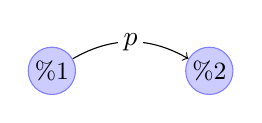
\begin{tikzpicture}
                    \tikzstyle{node}=[circle, draw=blue!50, fill=blue!20, inner sep=1pt, minimum size=6mm]
                    \tikzstyle{linenode}=[pos=0.5,fill=white,inner sep=2pt,outer sep=2pt]
                    \node[node] (A) at (0,0) {\small$\%1$};
                    \node[node] (B) at (2,0) {\small$\%2$};
                    \path [->] (A) edge[bend left] node[linenode] {$p$} (B);
                \end{tikzpicture}
            }
            \bitbox{29}[bgcolor=lightred]{Data} &
            \bitbox{1}[bgcolor=lightcyan]{\rotatebox{90}{Base}} &
            \bitbox{2}[bgcolor=lightgreen]{\rotatebox{90}{Next}}
        \end{rightwordgroup}
    \end{bytefield}
\end{center}
\begin{center}
    \definecolor{lightcyan}{rgb}{0.84,1,1}
    \definecolor{lightgreen}{rgb}{0.64,1,0.71}
    \definecolor{lightred}{rgb}{1,0.7,0.71}
    \begin{bytefield}[bitheight=\widthof{~Base~},
            boxformatting={\centering\small},rightcurly=., rightcurlyspace=0pt, bitwidth=11pt]{32}
        \bitheader{0-31} \\
        \begin{rightwordgroup}{Words}
            \bitbox{29}[bgcolor=lightred]{Data} &
            \bitbox{1}[bgcolor=lightcyan]{\rotatebox{90}{Base}} &
            \bitbox{2}[bgcolor=lightgreen]{\rotatebox{90}{Next}}
        \end{rightwordgroup}
    \end{bytefield}
\end{center}
\blindtext[1]

\subsection{Sparse Bitvectors}
\subsection{Memory Layout}
\subsubsection{Unified Memory}
\subsubsection{64bit Addresses}
\subsection{Concurrent Graph Rewriting}
\subsection{Integration with SVF}
\subsubsection{Parallelizing SVF}
\section{Experimental Results}
\subsection{Test Suite}
\subsection{Bemchmark Suite}
\section{Evaluation}
